% Options for packages loaded elsewhere
\PassOptionsToPackage{unicode}{hyperref}
\PassOptionsToPackage{hyphens}{url}
%
\documentclass[
]{book}
\usepackage{amsmath,amssymb}
\usepackage{lmodern}
\usepackage{ifxetex,ifluatex}
\ifnum 0\ifxetex 1\fi\ifluatex 1\fi=0 % if pdftex
  \usepackage[T1]{fontenc}
  \usepackage[utf8]{inputenc}
  \usepackage{textcomp} % provide euro and other symbols
\else % if luatex or xetex
  \usepackage{unicode-math}
  \defaultfontfeatures{Scale=MatchLowercase}
  \defaultfontfeatures[\rmfamily]{Ligatures=TeX,Scale=1}
\fi
% Use upquote if available, for straight quotes in verbatim environments
\IfFileExists{upquote.sty}{\usepackage{upquote}}{}
\IfFileExists{microtype.sty}{% use microtype if available
  \usepackage[]{microtype}
  \UseMicrotypeSet[protrusion]{basicmath} % disable protrusion for tt fonts
}{}
\makeatletter
\@ifundefined{KOMAClassName}{% if non-KOMA class
  \IfFileExists{parskip.sty}{%
    \usepackage{parskip}
  }{% else
    \setlength{\parindent}{0pt}
    \setlength{\parskip}{6pt plus 2pt minus 1pt}}
}{% if KOMA class
  \KOMAoptions{parskip=half}}
\makeatother
\usepackage{xcolor}
\IfFileExists{xurl.sty}{\usepackage{xurl}}{} % add URL line breaks if available
\IfFileExists{bookmark.sty}{\usepackage{bookmark}}{\usepackage{hyperref}}
\hypersetup{
  pdftitle={Environment},
  pdfauthor={Dyrehaugen Web Notebook},
  hidelinks,
  pdfcreator={LaTeX via pandoc}}
\urlstyle{same} % disable monospaced font for URLs
\usepackage{longtable,booktabs,array}
\usepackage{calc} % for calculating minipage widths
% Correct order of tables after \paragraph or \subparagraph
\usepackage{etoolbox}
\makeatletter
\patchcmd\longtable{\par}{\if@noskipsec\mbox{}\fi\par}{}{}
\makeatother
% Allow footnotes in longtable head/foot
\IfFileExists{footnotehyper.sty}{\usepackage{footnotehyper}}{\usepackage{footnote}}
\makesavenoteenv{longtable}
\usepackage{graphicx}
\makeatletter
\def\maxwidth{\ifdim\Gin@nat@width>\linewidth\linewidth\else\Gin@nat@width\fi}
\def\maxheight{\ifdim\Gin@nat@height>\textheight\textheight\else\Gin@nat@height\fi}
\makeatother
% Scale images if necessary, so that they will not overflow the page
% margins by default, and it is still possible to overwrite the defaults
% using explicit options in \includegraphics[width, height, ...]{}
\setkeys{Gin}{width=\maxwidth,height=\maxheight,keepaspectratio}
% Set default figure placement to htbp
\makeatletter
\def\fps@figure{htbp}
\makeatother
\setlength{\emergencystretch}{3em} % prevent overfull lines
\providecommand{\tightlist}{%
  \setlength{\itemsep}{0pt}\setlength{\parskip}{0pt}}
\setcounter{secnumdepth}{5}
\usepackage{booktabs}
\usepackage{amsthm}
\makeatletter
\def\thm@space@setup{%
  \thm@preskip=8pt plus 2pt minus 4pt
  \thm@postskip=\thm@preskip
}
\makeatother

\renewcommand\chaptername{}
\ifluatex
  \usepackage{selnolig}  % disable illegal ligatures
\fi
\usepackage[]{natbib}
\bibliographystyle{apalike}

\title{Environment}
\author{Dyrehaugen Web Notebook}
\date{2021-03-06}

\begin{document}
\maketitle

{
\setcounter{tocdepth}{1}
\tableofcontents
}
\hypertarget{environment}{%
\chapter{Environment}\label{environment}}

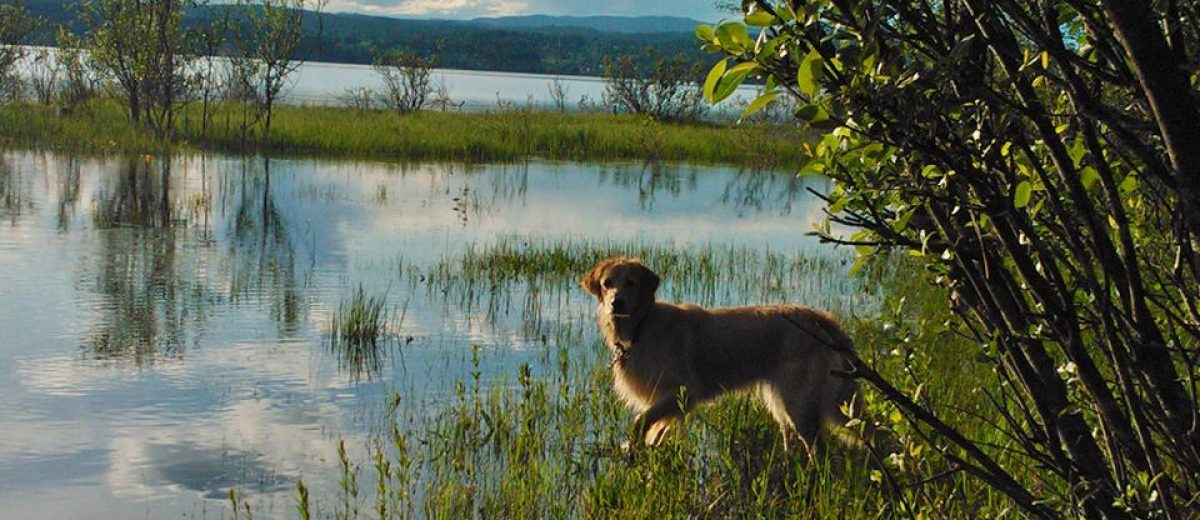
\includegraphics{fig/zelda.jpg}

Here we treat some major environmental issues.
You will not find \emph{Climate Change} here - it has got its own site/book.
The same applies to \emph{Development} i.e.~\emph{Capitalism} as the major
driver of environmental issues.
It too has got its own site/book.

\hypertarget{sustainability}{%
\chapter{Sustainability}\label{sustainability}}

\hypertarget{sustainability-issue-one}{%
\section{Sustainability Issue One}\label{sustainability-issue-one}}

\hypertarget{anthropocene}{%
\chapter{Anthropocene}\label{anthropocene}}

\hypertarget{material-footprint}{%
\section{Material Footprint}\label{material-footprint}}

\hypertarget{mfa}{%
\subsection{MFA}\label{mfa}}

\emph{Abstract Krausman:}
The growing extraction of natural resources and the waste and emissions
resulting from their use are directly or indirectly responsible for human-
ity approaching or even surpassing critical planetary boundaries. A sound
knowledge base of society's metabolism, i.e., the physical exchange pro-
cesses between society and its natural environment and the production and
consumption processes involved, is essential to develop strategies for more
sustainable resource use. Economy-wide material flow accounting (MFA) is
a framework that provides consistent compilations of the material inputs to
national economies, changes in material stocks within the economic system,
and material outputs to other economies and the environment. We present
the conceptual foundations of MFA and derived indicators and review the
current state of knowledge of global patterns and trends of extraction, trade,
and use of materials. We discuss the relation of material use and economic
development and the decoupling of material use from economic growth in
the context of sustainable resource use policies.

\hypertarget{eu28-footprint}{%
\subsection{EU28 Footprint}\label{eu28-footprint}}

\emph{Abstract Giljum:}
In the context of the transformation toward a ``green economy,'' issues related to natural
resource use have rapidly increased in importance in European and international policy
debates. The large number of studies applying economy-wide material flow analysis
so far mostly produced aggregated national indicators, making the results difficult to
connect to policies, which are often designed for single sectors or consumption areas.
This paper provides a detailed assessment of the composition of EU's material foot-
print in its global context, aiming at identifying the main product groups contributing
to overall material consumption and specifying the geographical sources for the raw
materials required to satisfy EU's final demand. Based on multi-regional input--output
(MRIO) modeling, we apply production layer decomposition to assess supply chains
and their structural changes from 1995 to 2011. The global MRIO database used in this
study is EXIOBASE 3, which disaggregates 200 products and 163 industries, of which 33
represent material extraction sectors. By that means, we increase the level of detail to
a degree where policies can more easily connect to. We find that the generally grow-
ing material footprint of the EU was characterized by a dramatic shift regarding the
origin of raw materials, with the share of materials extracted within the EU territory
falling from 68 \% in 1995 to 35 \% in 2011. In 2011, raw materials extracted in China to
produce exports to the EU already contributed an equal share to EU's material footprint
as material extraction within the EU itself. Import dependency is most critical for the
material group of metal ores, with only 13 \% of all metals required as inputs to EU final
demand stemming from within the EU. Regarding product composition, construction
was confirmed as the most important sector contributing to the material footprint, fol-
lowed by the group of manufacturing products based on biomass. Materials embodied
in service sector activities together contributed a quarter to the total material footprint
in 2011, making services an important, but currently disregarded area for European
resource policies. We also find that supply chain structures became more complex over
time, with a growing part located outside the EU territory.

\href{https://www.annualreviews.org/doi/10.1146/annurev-environ-102016-060726}{Krausman (2017) MFA Material Flow Accounting}
\href{pdf/Krausman_2017_MFA.pdf}{(pdf)}

\href{https://journalofeconomicstructures.springeropen.com/articles/10.1186/s40008-016-0048-5\#Abs1}{Giljum (2016) MRIO Based Material Footprint Assessment}
\href{pdf/Giljum_2016_MRIO_based_Material_Footprint.pdf}{(pdf)}

Max Roser tweeted the following text: ``Material Footprint' is a terrible metric, but it is unfortunately used as one of the indicators of the UN's Sustainable Development Goals. A metric that allows you to offset the use of a ton of coal by using one less ton of sand should really not have that status.'' (1) In the following discussion he said that we should: ``stop reporting environmental impact in this way.'' (2) and that he finds ``Equal weights for fossil fuels and stones {[}\ldots{]} ethically absolutely horrible.'' (3) To make this point, he referred to a recent publication, comparing and disaggregating the EU's overall material footprint (MF) between 1995 and 2011, and more specifically, to one apparent substitution of clay and sand (decreased) with coal use (increased by roughly the same amount)

`Material Footprint' seems to me a bad metric for our impact on the environment.
Some resource use is much more harmful and to treat a kg of sand just like a kg of coal is a terrible idea.
To simply sum up their weight hides that resource use that has the worst impact.

The usefulness of aggregate material flow indicators: their purpose is to study the social metabolism, which is the material scale, composition, and pattern of the human-environment interaction

f we look beyond Roser's blanket rejection of MF and at available scientific publications, we find that MF is actually a useful proxy for aggregate environmental pressures. This is simply because all material extraction (be it biomass, metals, fossil fuels or non-metal minerals) has some impact (7). So, if we measure MF and environmental impacts separately, we would expect to find a correlation between the two. This is exactly what happens. MF is highly correlated with other indicators for environmental pressure, such as carbon dioxide and ecological footprint (6). Also, as Krausmann et al.~state (8, see also 9), material use (here domestic) correlates well with more complex indicators such as environmentally-weighted material use, accounting for different impacts of the respective material categories. Another reason why MF is a useful indicator is its simplicity while being representative.
Indeed, Steinmann et al.~(10) assessed 976 products and found that (p.~1) ``the resource footprints {[}here material (excl. energy and biomass), energy, land, and water{]} accounted for \textgreater90\% of the variation in the damage footprints. {[}\ldots{]} Our results indicate that relatively simple resource footprints are highly representative of damage to human health and biodiversity''. Finally, Voet et al.~(11) reach similar conclusions (p.~130): ``if we compare environmental impact with DMC {[}Domestic Material Consumption{]}, we can conclude that the contribution to the environmental pressure and the contribution to the DMC is not so different for these {[}resource{]} categories''. Thus, MF captures important connections between human extractive activity and environmental pressures quite well on an aggregate level, and this in a simple and understandable way.

\href{https://degrowth.org/2021/02/06/aggregate-material-footprint-as-a-proxy-for-environmental-pressures/}{Lorenz Keyser - Reply to Max Roser}

\citep[ Twitter Thread]{LorenzClimate}(\url{https://twitter.com/LorenzClimate/status/1357810876410175492})

\hypertarget{global-human-made-mass-exceeds-all-living-biomass}{%
\subsection{Global human-made mass exceeds all living biomass}\label{global-human-made-mass-exceeds-all-living-biomass}}

\emph{Memo:}

At the beginning of the twentieth century, anthropogenic mass was equal to only 3\% of global biomass.
About 120 years later, in 2020, anthropogenic mass is exceeding overall biomass in the world.

As the global effect of humanity accelerates, it is becoming ever more imperative
to quantitatively assess and monitor the material flows of our socioeconomic system,
also known as the socioeconomic metabolism.
This quantification is at the heart of the economy-wide material flow analysis framework,
under the field of industrial ecology, which is based on mass balance accounting.

Humanity has become a dominant force in shaping the face of Earth.
We are in the Anthropocene.
The overall living biomass on Earth currently equals approximately 1.1 teratonnes.
The anthropogenic mass has recently doubled roughly every 20years.
The Earth is exactly at the crossover point.
The antropogenic mass will surpass all other global living biomass in 2020.
Each week more than the bodyweight of all humans of antropogenic mass is produced.
This quantification of the human enterprise gives a mass-based quantitative and symbolic characterizatio

The global mass of of produced plastic is greater than the overall mass of all terrestrial and marine animals combined.

\begin{longtable}[]{@{}ll@{}}
\toprule
Living Biomass & Human-mademass \\ \addlinespace
\midrule
\endhead
Animals 4 Gt & Plastic 8 Gt \\ \addlinespace
Trees 900 Gt & Buildings 1100 Gt \\ \addlinespace
\bottomrule
\end{longtable}

The mass of humans is only about 0.01\% of global biomass.
Since the first agricultural revolution, humanity has roughly halved the mass of plant.
While modern agriculture utilizes an increasing land area for growing crops,
the total mass of domesticated crops (about 0.01 Tt)11 is vastly outweighed by
the loss of plant mass resulting from deforestation,forest management and other land-use changes.
These trends in global biomass have affected the carbon cycle and human health.
Additional human actions, including livestock husbandry, hunting and overfishing,
have also strongly affected the masses of various other taxa.

Continuous increases in anthropogenic mass, peaking at over 5\% per year,
mark the period immediately following World War II.
This period, frequently termed the `Great Acceleration',
is characterized by enhanced consumption and urban development

Quantifying the human appropriation of net primary production,
have focused on the allocation of the biosphere productivity flow for human usage.
The anthropogenic mass does not arise out of the biomass stock but from
the transformation of the orders-of-magnitude higher stock of mostly rocks and minerals.
In doing so, humanity is converting near-surface geological deposits into a socially useful form,
with wide implications for natural habitats, biodiversity, and various climatic and
biogeochemical cycles.

\href{https://www.nature.com/articles/s41586-020-3010-5.epdf?sharing_token=5BfrjXKSdktry3fKS7ssCdRgN0jAjWel9jnR3ZoTv0MLvUZ1C0L35yEQYHf_pwmiKx-xqIzWDg-_bH8WmUJdQjqDv1hJIWjUwOgpVde7Oc47mU9HfjoCpd8F0qewoXmjl6QNLlUMD2eeD21ompdgtw3j2FQ9z0hhBzCsqewC9BUQNhgBo5rYNFnTf9gTg419kTld3VXUhXOFlygv007wkcA8jVVlyrBd14KL3O0lNyCW54cq4jSFDWqF63iJKDWo_R6M1MFwDWk6OSU79I8W9ga2hbL-jY7gNoOR9LOhqUfR2c1P5oQrsITBs9UtutQEh--2BsxnLatS_s9_H68tUNKvlSYLF9xHfwWb-DXmoouJXov9L4EbWJH6itdSZHqa\&tracking_referrer=www.theguardian.com}{Nature article (shared pdf)}

\href{https://www.nature.com/articles/s41586-020-3010-5}{Nature web}

\href{https://github.com/milo-lab/anthropogenic_mass}{Github Code and Data}

\hypertarget{biodiversity}{%
\chapter{Biodiversity}\label{biodiversity}}

\begin{quote}
There is no way 8-10 billion people make it over the 2100 line with
half of plants \& insects at risk of extinction.
No way.
We're sawing through the trunk of the tree of life:
we will fall too.
(Julia Steinberger (Twitter))
\end{quote}

\hypertarget{economics-of-biodiversity}{%
\section{Economics of Biodiversity}\label{economics-of-biodiversity}}

\hypertarget{dasgupta-review-2021}{%
\subsection{Dasgupta Review 2021}\label{dasgupta-review-2021}}

The report proposes

\begin{verbatim}
- Recognising nature as an asset and  
- Reconsidering our measures of economic prosperity.
\end{verbatim}

Recommendations include:

\begin{verbatim}
- Making food and energy systems sustainable through technological innovations and policies that change prices and behavioural norms  
- Investing in programmes that provide community-based family planning  
- Expanding and improving access to protected areas  
- Implementing large-scale and widespread investment in nature-based solutions to address biodiversity loss  
- Introducing natural capital into national accounting systems.
\end{verbatim}

\href{https://www.bbc.com/news/science-environment-55893696}{Dasgupta Review (BBC)}

The Dasgupta Review is an independent, global review on the Economics of Biodiversity led by Professor Sir Partha Dasgupta (Frank Ramsey Professor Emeritus, University of Cambridge). The Review was commissioned in 2019 by HM Treasury and has been supported by an Advisory Panel.

\textbf{The Review calls for changes in how we think, act and measure economic success.}

The new framework presented by the Review sets out
how we should account for Nature in economics and decision-making.

The Review finds that humanity has collectively mis-managed its global portfolio of assets,
meaning the demands on nature far exceed its capacity to supply the goods and services
we all rely on.

\begin{quote}
Humanity must ensure its demands on nature do not exceed its sustainable supply and must increase the global supply of natural assets relative to their current level. For example, expanding and improving management of Protected Areas; increasing investment in Nature-based Solutions; and deploying policies that discourage damaging forms of consumption and production.
\end{quote}

.

\begin{quote}
We should adopt different metrics for economic success and move towards an inclusive measure of wealth that accounts for the benefits from investing in natural assets and helps to make clear the trade-offs between investments in different assets. Introducing natural capital into national accounting systems is a critical step.
\end{quote}

.

\begin{quote}
We must transform our institutions and systems -- particularly finance and education -- to enable these changes and sustain them for future generations. For example, by increasing public and private financial flows that enhance our natural assets and decrease those that degrade them; and by empowering citizens to make informed choices and demand change, including by firmly establishing the natural world in education policy.
\end{quote}

\emph{Reactionn from Mark Carney.}
Ecosystems that have more diverse natural assets are more productive, resilient and adaptable. Just as diversity within a financial portfolio reduces risk and uncertainty, greater biodiversity reduces risks and uncertainty within a portfolio of natural assets. As we awaken to the importance of natural capital, we need to place greater value on sustainability and biodiversity -- the precondition to solving the twin crises of biodiversity and climate.

\emph{Reactionfrom Christiana Figueres:}
It is less costly to conserve Nature than to restore it once it's damaged or degraded and provides the economic rationale for expanding and improving the management of protected areas. We can translate this idea into action by protecting 30\% of the planet by 2030. The Review lays the foundation for how to address the twin crises of biodiversity and climate.

\emph{Reaction from Andrew Haldane:}
Most of economics and economic policy has neglected the role of Nature and
underplayed the importance of biodiversity in protecting both Nature and, ultimately, us.

\emph{Reaction from James E. Hansen:}
Flourishing nature, restoration of a healthy climate, and economic well-being of all humanity can co-exist, but they require understanding. Dasgupta's Review helps us begin a journey, which will require decades.

\href{https://www.gov.uk/government/publications/final-report-the-economics-of-biodiversity-the-dasgupta-review/the-economics-of-biodiversity-the-dasgupta-review-reactions}{Dasgupta Review Reactions at Launch}

\textbf{Memo Dasgupta:}

While most models of economic growth and development recognise that Nature is capable only
of producing a finite flow of goods and services, the focus has been to show that technological
progress can, in principle, overcome that exhaustibility. This is to imagine that, ultimately,
humanity is `external' to Nature.
The Review develops the economics of biodiversity on the understanding that we -- and our
economies -- are `embedded' within Nature, not external to it. The Review's approach is based
firmly in what we know from ecology about how ecosystems function, and how they are
affected by economic activity, including the extraction of natural resources for our production
and consumption, and the waste we produce through these activities, which ultimately damages
ecosystems and undermines their ability to provide the services on which we rely. This approach
helps us to understand that the human economy is bounded and reshapes our understanding
of what constitutes truly sustainable economic growth and development: accounting fully for
the impact of our interactions with Nature and rebalancing our demand with Nature's capacity
to supply.

The change required should be geared towards three broad \textbf{transitions}:

\begin{enumerate}
\def\labelenumi{(\roman{enumi})}
\item
  Ensure that our demands on Nature do not exceed its supply,
  and that we \textbf{increase} (\emph{sic!!}) Nature's supply relative to its current level.
\item
  Change our measures of economic success to guide us on a
  more sustainable path.
\item
  Transform our institutions and systems -- in particular our
  finance and education systems -- to enable these changes and
  sustain them for future generations.
\end{enumerate}

Not so long ago, when the
world was very different from what it is now, the economic questions that needed urgent
response could be studied most productively by excluding Nature from economic models.
Nature entered macroeconomic models of growth and development in the 1970s, but in an
inessential form. 3 The thought was that human ingenuity could overcome Nature's scarcity over
time, and ultimately (formally, in the limit) allow humanity to be free of Nature's constraints.
But the practice of building economic models on the backs of those that had most recently been
designed meant that the macroeconomics of growth and development continued to be built
without Nature's appearance as an essential entity in our economic lives.

The natural world is studied in relation to the many other assets we
hold in our portfolios, such as the vehicles we use for transport, the homes in which we live,
and the machines and equipment that furnish our offices and factories. But like education and
health, Nature is more than a mere economic good. Nature nurtures and nourishes us, so we
will think of assets as durable entities that not only have use value, but may also have intrinsic
worth. Once we make that extension, the economics of biodiversity becomes a study in portfolio
management.

Finance plays a crucial role. A significant portion of the responsibility for helping us to shift
course will fall on the global financial system.

\textbf{To leave Nature alone so that it is able to thrive is to invest in it.}

The risks associated with biodiversity loss -- reductions in the productivity and resilience of
ecosystems along supply chains -- have significant macroeconomic and financial implications.
Far more global support is needed for initiatives directed at enhancing the understanding and
awareness among financial institutions of Nature-related financial risks, learning and building
on the advances on climate-related financial risks.

Central banks and financial supervisors can
support this by assessing the systemic extent of Nature-related financial risks. A set of global
standards is required. They should be underpinned by data that are both credible and useful for
decision-making. Businesses and financial institutions could then be obliged to integrate Nature-
related considerations with their other objectives. The idea ultimately is to have them assess
and disclose their use of natural capital. The Task Force on Nature-related Financial Disclosures,
(TNFD) established in 2020, is a step in that direction.

Integrating the protection of biodiversity with the fiduciary duties of
institutional investors and asset managers
would be a way to ensure their investment policies account for natural capital.

The time horizonwithin which financial actors plan and act is, unhappily (!!sic!!),
not more than a few years.
Financial regulators and supervisors can play a key role in the necessary shift
by changing their own assessment horizons and using their regulatory powers.

\emph{Moral Issue}
Ultimately though, it is we citizens who can bring about such changes. (!!sic!!)
Connecting with Nature needs to be woven throughout our lives.
The three pervasive features of Nature -- mobility, silence and invisibility --
mean that the consequences of actions
which desecrate Nature are often untraceable to those who are responsible.
We will have to rely also on self-enforcement, that is, be our own
judge and jury.

\textbf{Memo Main Report:}
Now we are plundering every corner of the world, apparently neither knowing or caring what
the consequences might be.

Today, we ourselves, together with the livestock we rear for
food, constitute 96\% of the mass of all mammals on the planet. Only 4\% is everything else --
from elephants to badgers, from moose to monkeys. And 70\% of all birds alive at this moment
are poultry -- mostly chickens for us to eat.

\emph{GDP}
The contemporary practice of using Gross Domestic Product (GDP) to judge
economic performance is based on a faulty application of economics. GDP is a flow (so many
market dollars of output per year), in contrast to inclusive wealth, which is a stock (it is the
social worth of the economy's entire portfolio of assets). Relatedly, GDP does not include the
depreciation of assets, for example the degradation of the natural environment (we should
remember that `G' in GDP stands for gross output of final goods and services, not output net
of depreciation of assets). As a measure of economic activity, GDP is indispensable in short-run
macroeconomic analysis and management, but it is wholly unsuitable for appraising investment
projects and identifying sustainable development. Nor was GDP intended by economists who
fashioned it to be used for those two purposes. An economy could record a high rate of
growth of GDP by depreciating its assets, but one would not know that from national statistics.

\textbf{VALUES}
Correct economic reasoning is entangled with our values. Biodiversity does not only have
instrumental value, it also has existence and intrinsic value, perhaps even moral worth.

\textbf{(Use) Value} vs \textbf{(Intrinsic) Worth} vs \textbf{(Social) Worth} vs \textbf{(Inclusive) Wealth}
Nature is more than a mere economic good. Nature nurtures and nourishes us,
so we will think of assets as durable entities that not only have use value, but may also have
intrinsic worth. Once we make that extension, the economics of biodiversity becomes a study in
portfolio management.

In order to judge whether the path of economic development
we choose to follow is sustainable, nations need to adopt a system of economic accounts that
records an inclusive measure of their wealth. \textbf{The qualifier \emph{inclusive} says that wealth includes
Nature as an asset.}

The contemporary practice of using Gross Domestic Product (GDP) to judge
economic performance is based on a faulty application of economics. GDP is a flow (so many
market dollars of output per year), in contrast to inclusive wealth, which is a stock (it is the
social worth of the economy's entire portfolio of assets)

\emph{Inclusive Wealth}
The accounting value of an economy's stock of capital goods is its inclusive wealth. The qualifier
signals that the notion of wealth adopted here differs from the one in common use in two ways:
(i) accounting prices are not necessarily market prices; and (ii) in addition to produced capital,
wealth includes human capital and natural capital. As accounting prices measure the social
worth of goods and services, the inclusive wealth of a nation is the social worth of its capital
goods. As noted previously, by `social worth' we mean not only the worth to people who are
alive at that date, but also to future people.

\textbf{Valueing Biodiversity}
Ecosystems are capital goods. Biodiversity is a characteristic of ecosystems. In the terminology
introduced in Chapter 1, it is an enabling asset.

Humanity's future will be shaped by the portfolio of \textbf{assets} we inherit and choose to pass on,
and by the balance we strike between the portfolio and the size of our population. \emph{Assets are
durable objects, producing streams of services}. Their durability enables us to save them for our
own future, offer them as gifts to others, exchange them for other goods and services, and
bequeath them to our children. Durability does not mean everlasting. Assets depreciate, but
unlike services they are not fleeting.

\emph{Capital Assets}
Perhaps because financial capital has figured prominently in
economists' writings, the qualifier `capital' is sometimes added to assets, as in `capital assets'.
Assets acquire their value from the services they provide over their remaining life

\emph{Wealth Accounts}
a deep connection
between inclusive wealth and intergenerational well-being. We prove that any change in one
is mirrored in a corresponding change in the other. The correspondence is named the wealth/
well-being equivalence theorem. We show that the theorem offers a way to judge whether the
development path an economy is following meets the requirement of sustainability. The theorem
is also shown to be the right criterion for evaluating public policy. Inclusive wealth is the coin
with which economic progress or its absence should be measured. Private companies prepare
balance sheets. The theorem shows why countries should now prepare wealth accounts.

\textbf{Capital Goods} vs \textbf{Enabling Assets}
In our classification, there are thus three categories of capital goods and
a wide range of enabling assets.
Three-way partition of \emph{capital goods}: produced capital (buildings, roads,
ports, machines, instruments), human capital (population size, health, education, reputation,
knowledge and skills) and natural capital (ecosystems, sub-soil resources).
What remains -- institutions and practices, more generally, social capital, and
publicly available knowledge --
we will call \emph{enabling assets},
because they confer value to the three classes of capital goods by facilitating their use.

** Economic Evaluation**
Management of a society's portfolio of assets involves
policy analysis and
sustainability assessment.
We call the two generically as economic evaluation.

\emph{(Green Book 6.48)}
A focus solely on the marginal valuation of a loss in services may overlook the potential
for large reductions in stocks.

\emph{Pollinators}
At smaller levels of aggregation, total values of Nature's services can be meaningful and yet not
be useful for policy. It is tempting, for example, to cite the estimate that pollination contributes
an annual £510-690 million to the UK's agricultural production as providing a reason for
restoring the population of pollinators (Breeze, Roberts, and Potts, 2012). But should we regard
it to be a large or small figure? Based on 2019 data from the UK Office of National Statistics,
as a proportion of the UK's annual agricultural output, it is approximately 5\%. As a proportion
of the UK's GDP, it is 0.03\%, a negligible figure. So why care whether any pollinators are left?
The reason we should not be dismissive of pollinators is that proportional figures do not signal
worth. National asset management requires that pollinators enter projects with their accounting
prices. Chapters 2 to 4 demonstrate that pollinators may be of great value even if their
measurable services to GDP are of negligible worth.

\href{https://www.gov.uk/government/publications/final-report-the-economics-of-biodiversity-the-dasgupta-review}{Dasgupta Review Final Report}
\href{pdf/Dasgupta_2021_Final.pdf}{(pdf final (full) report)}
\href{pdf/Dasgupta_2021_Short.pdf}{(pdf short)}
\href{pdf/Dasgupta_2021_Messages.pdf}{(pdf messages)}
\href{pdf/Dasgupta_2021_Interim.pdf}{(pdf Interim Report (April 2020))}

\href{https://tnfd.info/}{TNFD}

\textbf{Observations}

Borgelig idealisme

Document Searches:
`capitalism': 2 entries\\
`doughnut': 0

\hypertarget{habitat-loss}{%
\chapter{Habitat Loss}\label{habitat-loss}}

\hypertarget{food-industry-drives-habitat-loss}{%
\section{Food industry drives habitat loss}\label{food-industry-drives-habitat-loss}}

\emph{Memo}

The projected loss of millions of square kilometres of natural ecosystems to meet
future demand for food, animal feed, fibre and bioenergy crops is likely to
massively escalate threats to biodiversity.
Proactive policies targeting how, where, and what food is produced could reduce these threats, with a combination of approaches potentially preventing almost all these losses while contributing to healthier human diets.

The global food system is on course to drive rapid and widespread ecological damage with almost 90\% of land animals likely to lose some of their habitat.
Without fundamental changes, millions of square kilometres of natural habitats could be lost by 2050.

While conventional conservation tactics such as establishing new protected areas
or introducing legislation to save specific species were necessary,
the research underscored the importance of ``reducing the ultimate
stresses to biodiversity -- such as agricultural expansion''.

Shifting to healthier diets would have big benefits in North America, but it is less likely to have a large benefit in regions where meat consumption is low and food insecurity is high.

Responding to the impending biodiversity crisis requires decisions informed by high-resolution,
spatially explicit and species-specific assessments of many thousands of species
to identify the species and landscapes most at risk.
Results from these assessments can be used to help plan appropriate conservation responses,
such as species- or location-specific legislation, and to assess which proactive changes
to food systems have the greatest potential to reduce future threats to biodiversity before
they occur.
The utility of most existing analyses for conservation planning and action has been limited by
coarse spatial resolutions, a focus on a relatively small suite of species or
on generalized biodiversity metrics such as species richness,
or using narrative pathways that are neither tied to current agricultural trajectories
nor able to examine how specific changes to food systems might mitigate future biodiversity declines.

{[}The new research{]} analyse at a high spatial resolution (1.5 × 1.5 km)
the impacts of likely agricultural expansion
on an unprecedented number of species (almost 20,000)
while explicitly accounting for differences in how individual species may be impacted
by agricultural land-use change,
and by analysing how proactive food-system transitions might mitigate future biodiversity decline.

The projected severity of agricultural land-cover change on habitat area means that proactive policies to reduce future demand for agricultural land will probably be required to mitigate widespread biodiversity declines. To investigate the potential of such proactive approaches, we developed a scenario that implemented four changes to food systems: closing crop yield gaps globally, a global transition to healthier diets, halving food loss and waste, and global agricultural land-use planning to avoid competition between food production and habitat protection.

In reality, threats to biodiversity could be considerably greater than those we project: other projections of future agricultural land demand are higher than those we use5, and we do not include the impacts of anthropogenic climate change, habitat fragmentation, over-exploitation, invasive species or pollution5,6,39--41. Climate change is likely to drive widespread changes in biodiversity by altering the location of suitable habitats and environments, and may have synergistic effects with habitat loss and fragmentation from agricultural expansion41. In addition, its effect on agricultural yields42 and the relative suitability of different regions for various crops43 could have indirect impacts on biodiversity by altering patterns of agricultural expansion. Uncertainty in how climatic changes will affect agriculture44 and species45 precludes quantitatively assessing these impacts

\href{https://www.theguardian.com/environment/2020/dec/21/global-food-industry-to-drive-rapid-habitat-loss-research}{Food Industry drives habitat loss (Guardian)}

\href{https://www.nature.com/articles/s41893-020-00656-5.epdf?sharing_token=R2MS-n7EpYm6CQn6PyyqL9RgN0jAjWel9jnR3ZoTv0O6RrkjpmW9fP_y1r0KlZ-Jx6UWX_jcBOXnlP2cYuEslvZu1-m7EgvCszD8mx-fwAIyiIh3Gx1tvRg-Geb5oZYMrgHYywVW7ovXIyZGEpuBr79zSzsD8wwHk_mBt8B8l1kD4xX_vLU2HtS04lrY7S9dTPE2uBW6UFWvOPGd3COAVQjH2qEEkkmbXzsW9f9DQh3JSJxMsDCiFz84VmI_GLPqG-tl6sb70A-DTfHoDYnqvlncEQlHNJLKvMauKaoH-1acinO7dw5-2OW3LzB2QDW-3G7YVVO3x8J2MOFAfUTTGlrNf0ZNDDvSOygvJ1S5z0E6Chteld_Pgugf-yhbLXH9t5TkqNaBYlrrKXb-bgmBYr68yQbKOcBwQy7EfcgOgAnmIVbitCX94Y-_DdD00Vp3YRsOm9AhIG2fmkWzW8OY4nB4Bi2BafrHNNHniHbTJidRx5Uxm8_GFX9tykH3e_M00qDlLJhxMWq1Tl45zu6vdQ\%3D\%3D\&tracking_referrer=www.theguardian.com}{Nature article (shared pdf)}

\href{https://www.nature.com/articles/s41893-020-00656-5}{Nature article (web))}

\hypertarget{mass-extinction}{%
\chapter{Mass Extinction}\label{mass-extinction}}

\hypertarget{coral-reefs}{%
\section{Coral Reefs}\label{coral-reefs}}

Bad news from the Coral Reefs.
Bleaching is going on and reefs are not healing between events
UNEP is reporting on this issue.

From the 2020 report:

\begin{quote}
Stony corals bleach when warm sea temperatures disrupt the mutualistic relationship between
the algal symbionts, called zooxanthellae, that reside within the host coral tissues (Douglas
2003). Corals can either regain their zooxanthellae (Baker 2001) and survive or die if
temperature stress persists. The third global coral bleaching event, which started in 2014 and
extended well into 2017, was the longest coral bleaching event on record (Eakin et al.~2019).
The length of the event means corals in some parts of the world had no time to recover in 2014,
2015 or 2016 during the cool/winter season, prior to experiencing bleaching the following year.
Van Hooidonk et al.~(2013, 2014, 2016 and 2017) found that a majority of coral reefs are
projected to experience annual severe bleaching (ASB) by the mid-2040's under a business-as-
usual emissions scenario (RCP8.5). This means that the recent global bleaching event of 2014-
2017 represents what climate models suggest may become the norm over the coming few
decades. Lower frequencies of bleaching events per decade (e.g., 2x or 4x per decade) are
projected to occur earlier than ASB. ASB is projected here because annual severe bleaching is a
time beyond which coral reefs seem certain to change (and possibly rapidly degrade).
Importantly though, great spatial variation exists in the projected timing of the onset of ASB
conditions among the world's coral reefs. This variation will be a major driver of differences in
the relative vulnerability of coral reef ecosystems to climate change.
\end{quote}

\begin{quote}
In the IPCC's widely adopted vulnerability assessment framework, vulnerability is a function of
exposure to climate and non-climate threats and sensitivity to these threats, which yields
potential impacts that are moderated by adaptive capacity (Turner et al.~2003). Sensitivity and
adaptive capacity can be collectively seen as resilience (Marshall and Marshall 2007), i.e., the
capacity of a system to absorb or withstand stressors such that the system maintains its
structure and functions in the face of disturbance and change, and the capacity to adapt to
future challenges (McLeod et al.~2019). Managing coral reefs for resilience entails reducing
coral reef vulnerability to climate change by reducing exposure to non-climate threats (i.e., local-
scale anthropogenic stress, Anthony et al.~2014).
\end{quote}

\begin{quote}
A key challenge for reef management lies in deciding where to target actions to reduce
anthropogenic stress, ensuring efficacy as well as cost effectiveness of actions taken.
Ecosystem and Resilience Based Management (EBM and RBM) are becoming increasingly
sophisticated (Mills et al.~2015, McLeod et al.~2019), and software that combines and analyzes
spatial data is increasingly accessible and used in planning to strike a balance between what
can be competing conservation and development objectives (Watts et al.~2009). For example,
protecting biodiversity, providing for sustainable fisheries, and minimizing user conflicts are
among the highest priorities during marine spatial planning (MSP) efforts in reef areas (Agardy
et al.~2011). Incorporating spatial variation in coral reef vulnerability to climate change is
frequently discussed during MSP but, as yet, is rarely operationalized (Anthony et al.~2014). This
will require assessing spatial variation in the key vulnerability components -- exposure and
resilience - at a locally relevant scale (one km to 10s of km).
\end{quote}

\href{https://www.unenvironment.org/resources/report/coral-bleaching-futures}{UNEP Coral Bleaching Futures 2017}
\href{/pdf/UNEP_2017_Coral_Bleaching_Futures.pdf}{(pdf)}

\href{https://www.unenvironment.org/resources/report/projections-future-coral-bleaching-conditions-using-ipcc-cmip6-models-climate}{UNEP Coral Reefs Report 2020}
\href{/pdf/UNEP_2020_Coral_Reefs_CMIP6.pdf}{(pdf)}

\href{https://www.cell.com/trends/ecology-evolution/fulltext/S0169-5347(20)30306-2\#secst0025}{Biological Conservation Issues 2021 Scanning}

\hypertarget{pollution}{%
\chapter{Pollution}\label{pollution}}

\hypertarget{fertility}{%
\section{Fertility}\label{fertility}}

Following current projections, the median sperm count is set to reach zero in 2045.

\href{https://www.theguardian.com/us-news/2021/feb/26/falling-sperm-counts-human-survival}{The Guardian}

\hypertarget{plastics}{%
\section{Plastics}\label{plastics}}

\hypertarget{finance}{%
\subsection{Finance}\label{finance}}

\emph{Memo}

To address plastic pollution, a fundamental shift
away from business models that depend on sin-
gle-use packaging towards those that prioritise
reuse and more localized supply chains and services
is needed.
Banks should make funding of corporate
actors within the plastic packaging supply
chain contingent on companies implement-
ing best practice.
Governments should stop protecting banks
and re-write the rules of finance to hold
banks liable for the damage caused by their
lending.
Companies must adopt international best
practice to reduce the production and use
of virgin plastic and increase the reusability
of plastic packaging products.

Banks are silent and out of touch
with reality
This global public outcry led to a set of govern-
ment and business responses. As of June 2020, it
was reported that 69 countries had passed a full or
partial ban on plastic bags. Some companies have
made comparatively strong commitments to reduce
plastic packaging. Despite public outcry over the serious impacts
of plastic pollution, and efforts by some companies
within the plastic value chain to reduce their impacts,
none of the banks analysed have developed due
diligence systems, contingent loan criteria or financ-
ing exclusions when it comes to this industry. This
means banks are currently not taking responsibility
to understand, measure, and reduce the impacts of
their loans within the plastics value chain.
By indiscriminately funding actors in the plastic
supply chain, banks have failed to acknowledge
their role in enabling global plastic pollution. They
have fallen far behind the crowd of other actors that
contribute to the plastic pollution crisis.

By indiscriminately funding actors in the plastic
supply chain, banks have failed to acknowledge
their role in enabling global plastic pollution.
They have fallen far behind other actors that
contribute to the plastic pollution crisis.

The concentration of finance
from banks Headquarted in
a few jurisdictions indicates
that legislative measures, such
as introducing lender liability
which holds financiers and
investors responsible for the
impacts their financing has on
biodiversity, could be highly
impactful even when initially
implemented in a small number
of geographic regions.

A limited number of banks have started to adopt
policies that allow them to limit investments for other
high biodiversity impacting sectors such as fossil
fuels, forest products, and some agricultural commod-
ities. However, this has not yet occurred for plastics.

Governments and financial institutions
should both recognise that investment in the plastics
supply chain without sufficient investment in the
plastics value recovery chain (reduction, recovery,
re-use and recycling), causes and contributes to this
harm. To remedy the problem, governments should:

Extend investor liability for any future envi-
ronmental or health related legal challenges
to those responsible for plastic pollution,
especially effects of it entering the food
chain.

Introduce a mandatory tax on virgin plastic
at the point of importation to or production
within a country, in order to raise its price
relative to recycled plastics, achieving
equivalence by channeling the receipts from
the tax into incentives to recover and reuse
plastics waste streams. This would require
trade related controls to ensure equivalence
in imported packaging.

Invest in a new generation of recycled
plastics markets by establishing forward
contracting arrangements akin to renew-
able energy feed in tariffs to incentivise
investment in modern recycled plastics
value chains.

\href{https://portfolio.earth/campaigns/bankrolling-plastics/}{Portfolio.earth Bankrolling Plastics}

\hypertarget{pandemics}{%
\chapter{Pandemics}\label{pandemics}}

\hypertarget{loss-of-habitat-as-a-driver}{%
\section{Loss of habitat as a driver}\label{loss-of-habitat-as-a-driver}}

Som text on the linksbetween loss of biodiversity and pandemics

\begin{quote}
Almost all pandemics start with a single infection event. For zoonoses from wildlife, this is a person, or group of people that made contact with an animal infected by a pathogen that infects them, replicates in their cells and then is transmitted to others. Surveillance data suggest that spillover events happen frequently around the world, but most infections are unable to cause further transmission among people. Sometimes, pathogens spill over and are able to transmit to a handful of people, undergoing a few cycles of transmission before the outbreak dies out. Where pathogens spread into dense human communities (e.g.~COVID-19 within the live animal market and city of Wuhan 10 ), and when they are able to easily transmit from person-to-person, they can become pandemics. Preventing pandemics will require efforts to reduce the risk each of these stages occurring, through measures that diminish the underlying drivers of spillover, their spread among people and their ability to move globally through rapidly urbanizing landscapes, megacities and travel and trade networks.
\end{quote}

\begin{quote}
Pandemics represent an existential threat to the health and welfare of people across the planet, and their emergence, impact and control are deeply embedded in biodiversity and the major causes of biodiversity loss. New diseases emerge largely in tropical or subtropical countries with high wildlife biodiversity. The first people to be infected are often from communities in remote or rural regions, in developing countries with lower capacity to rapidly diagnose and treat novel diseases, and control and contain pandemic spread. Land use change and the wildlife trade (especially unsustainable, illegal or poorly regulated wildlife trade) are key drivers of pandemic emergence, including the recent emergence of COVID-19. Pandemics, such as COVID-19, underscore both the indivisible interconnectedness of the world community and the rising threat posed by global inequality to the health, wellbeing and security of all people: Exponential growth in consumption of products from land use change and globalized trade, often driven by developed countries, have led to the repeated emergence of diseases from developing countries with high biodiversity, and thus conditions that increase potential for zoonotic emergence.
\end{quote}

\hypertarget{bats-habitat-loss-drives-diseases}{%
\subsection{Bats habitat loss drives diseases}\label{bats-habitat-loss-drives-diseases}}

Many of the recently emerging highly virulent zoonotic diseases have a
likely bat origin, for example Hendra, Nipah, Ebola and diseases caused
by coronaviruses.
Presumably because of their long history of coevolution, most of these
viruses remain subclinical in bats,
but have the potential to cause severe illnesses
in domestic and wildlife animals and also humans.

Increasing numbers of breakouts of zoonotic viral diseases among
humans and livestock have mainly been accounted to human encroachment
into natural habitat, as well as agricultural intensification,
deforestation and bushmeat consumption.
Persecution of bats, including the destruction of their roosts and culling of
whole colonies, has led not only to declines of protected bat species,
but also to an increase in virus prevalence in some of these populations.

\href{https://www.researchgate.net/publication/286449572\%20_Zoonotic_Viruses_and_Conservation_of_Bats}{Zoonotic Diseases and Conservation of Bats}
\href{/pdf/Schneeberger_Voigt_2016_Bats_Zoonotic.pdf}{(pdf)}

\href{https://www.bbc.com/future/article/20210106-nipah-virus-how-bats-could-cause-the-\%20next-pandemic}{Nipah (BBC)}

\hypertarget{apolitical-public-health}{%
\section{Apolitical Public Health}\label{apolitical-public-health}}

\emph{Memo}

Global health is a discipline that holds within itself a deep contradiction---global health was birthed in supremacy, but its mission is to reduce or eliminate inequities globally.

Most epidemiological analyses and modeling studies to be devoid of any analyses of power. ``For the most part, epidemiology as a method of science is considered apolitical; it actually serves as an ideological apparatus of imperialism by shielding structural causes of health inequities in the Global South,''

Epidemiological analyses of disease dynamics that fail to consider sociohistorical forces. In doing so, these studies end up diverting the public's gaze from legacies of colonialism, white supremacy, structural adjustment, institutional racism, and purposeful under-development which leaves health systems so weak and ineffective.

Move away from the notion of a universal truth.
Reject the notion that social inquiry can produce objective, value-neutral, and univocal understanding. Instead, we must embrace the critical and the polyvocal.

\href{https://naturemicrobiologycommunity.nature.com/posts/a-mind-bending-take-on-the-coloniality-of-global-public-health}{Epidemic Illusions}

\hypertarget{pandemic-risk-management}{%
\section{Pandemic Risk Management}\label{pandemic-risk-management}}

\emph{Memo}

We are dealing with an extreme fat-tailed process owing to an increased connectivity,
which increases the spreading in a nonlinear way.
Fat tailed processeshave special attributes, making conventional risk-management
approaches inadequate.

The general (non-naive) precautionary principle delineates conditions where actions
must be taken to reduce risk
of ruin, and traditional cost-benefit analyses must not be used.
These are ruin problems where, over time, exposure to tail
events leads to a certain eventual extinction. While there
is a very high probability for humanity surviving a single
such event, over time, there is eventually zero probability of
surviving repeated exposures to such events. While repeated
risks can be taken by individuals with a limited life expectancy,
ruin exposures must never be taken at the systemic and
collective level. In technical terms, the precautionary principle
applies when traditional statistical averages are invalid because
risks are not ergodic.

Estimates of the virus's reproductive
ratio \$R\_\{0\} - the number of cases one case generates on average
over the course of its infectious period in an otherwise
uninfected population - are biased downwards. This property
comes from fat-tailedness {[}4{]} due to individual `superspreader'
events. Simply, R 0 is estimated from an average which takes
longer to converge as it is itself a fat-tailed variable

Standard individual-scale policy approaches
such as isolation, contact tracing and monitoring are rapidly
(computationally) overwhelmed in the face of mass infection,
and thus also cannot be relied upon to stop a pandemic. Multi-
scale population approaches including drastically pruning con-
tact networks using collective boundaries and social behavior
change, and community self-monitoring, are essential.
Together, these observations lead to the necessity of a
precautionary approach to current and potential pandemic
outbreaks that must include constraining mobility patterns in
the early stages of an outbreak, especially when little is known
about the true parameters of the pathogen.
It will cost something to reduce mobility in the short term,
but to fail do so will eventually cost everything---if not from
this event, then one in the future. Outbreaks are inevitable, but
an appropriately precautionary response can mitigate systemic
risk to the globe at large. But policy- and decision-makers must
act swiftly and avoid the fallacy that to have an appropriate
respect for uncertainty in the face of possible irreversible
catastrophe amounts to ``paranoia,'' or the converse a belief
that nothing can be done.

\href{https://necsi.edu/systemic-risk-of-pandemic-via-novel-pathogens-coronavirus-a-note}{Norman/Bar-Yam/Taleb Note}
\href{/pdf/Joseph_Norman_2020_Systemic_Risk_of_Pandemic_via_Novel_Pathogenes.pdf}{(pdf)}

\hypertarget{land-use}{%
\chapter{Land Use}\label{land-use}}

\hypertarget{agriculuture}{%
\section{Agriculuture}\label{agriculuture}}

Our industrial food boom spawned similar failures of systemic context. Our inventive, so-called green revolution of food solutions produced a lot of food and made profits for large corporations, but depleted soil nutrients, spread toxins, severed mycelial networks, and disrupted nutrient cycles, creating eutrophic lakes and dead zones in our oceans.

\href{https://mahb.stanford.edu/blog/thresholds-cascades-and-wicked-problems/}{Wicked Complexity}

\hypertarget{forests}{%
\section{Forests}\label{forests}}

\hypertarget{lakes}{%
\section{Lakes}\label{lakes}}

\hypertarget{mountains}{%
\section{Mountains}\label{mountains}}

\hypertarget{urban}{%
\section{Urban}\label{urban}}

\hypertarget{actions}{%
\chapter{Actions}\label{actions}}

\hypertarget{analysis}{%
\section{Analysis}\label{analysis}}

I remember thinking, in the 1970s, that once people became aware of the ecological crisis --- disappearing species, polluted rivers, poisoned air --- that the necessary changes would be simple to achieve. Humanity only had to curb industrial waste and destruction, preserve wilderness for other species, put limits on our consumption, stabilize human population, and just be smart about how to live on Earth without destroying it.

Of course, I was naive to think any of that would be easy. Since that time, human population has doubled, consumption of material resources has quadrupled, biodiversity collapse has accelerated, and after 34 international climate meetings, we are emitting more carbon than ever before. Meanwhile, we have not exactly ended war, vanquished racism, nor achieved gender or economic parity. Even worse, giant corporate interests actively work to halt and reverse any ecological regulation on industrial activity.

Our emotional responses to crisis evolved over millennia, primarily to meet immediate needs, perhaps to benefit our tribe or community, not necessarily to solve complex, multi-dimensional, long-term dilemmas. Our ideas about ``solutions'' tend to be linear, short-term, and linked to a perception of simple cause and effect. Our educational institutions encourage this linear thinking about problems and solutions. Meanwhile, our social and ecological challenges are systemic, multidimensional, and complex.

Living ecosystems are dynamic, always changing, and possess qualities such as thresholds, cascades, feedback loops, tipping points, lags, and generally unintended consequences to input. Maybe we need to learn more about how change actually occurs in nature, not just in our imaginations or in our engineering dissertations.

\href{https://mahb.stanford.edu/blog/thresholds-cascades-and-wicked-problems/}{Wicked Complexity}

\hypertarget{actionism}{%
\section{Actionism}\label{actionism}}

\begin{quote}
Any activist group needs a sound theory of change and a clear strategy for gaining influence.
\end{quote}

\href{https://jacobinmag.com/2020/12/climate-change-protest-strategy-electoral-politics-sunrise-extinction-rebellion}{Organizing Actions (Edward Carver on Sunrise and XR)}

\hypertarget{bankrolling}{%
\section{Bankrolling}\label{bankrolling}}

\emph{Bankrolling} is about making finance institutions responsible for the environmental
impacts of what they finance.

\hypertarget{bankrolling-plastics}{%
\subsection{Bankrolling Plastics}\label{bankrolling-plastics}}

Banks are failing to address the global plastic-pollution crisis,
having provided \$1.7 trillion in financing to packaging companies, retailers and
related businesses.

The banks haven't put in place due-diligence processes for packaging companies or
made funding contingent on policies that reduces plastic and favors recycling
over virgin plastics.

Banks are currently not taking any responsibility to understand, measure or reduce
the impacts of their loans within the plastics value chain.
By indiscriminately funding actors in the plastics supply chain, banks have failed
to acknowledge their role in enabling global plastic pollution.

Banks need to mitigate their role in enabling plastic pollution in a number of ways
-- for example, by aligning their lending portfolios with public policy
on plastic reduction, reusability and recycling,
and ceasing the financing of new plants that use virgin feedstock
to produce single-use plastic packaging.

\href{https://www.bloomberg.com/news/articles/2021-01-07/banks-directed-1-7-trillion-to-firms-causing-plastic-pollution}{Bloomberg News}

\href{https://portfolio.earth/}{Portfolio Earth}

\hypertarget{bankrolling-extinction}{%
\section{Bankrolling Extinction}\label{bankrolling-extinction}}

\emph{Memo}

It is clear banks
do not consider
themselves
responsible
or liable for
biodiversity
impacts caused
by their lending
activities

In 2019 the world's largest banks invested more than USD 2.6 trillion (equivalent to Canada's GDP) in sectors governments and scientists agree are the primary drivers of biodiversity destruction.

The financial sector is bankrolling the mass extinction crisis, while undermining human rights and indigenous sovereignty.

We are currently in the midst of a mass
extinction event. Termed the `Anthropocene
Extinction', this is the first of its kind to be
caused by humans. Humans have impacted
nearly every corner of the planet and are
approaching planetary boundaries which
could take millions of years to recover
from. 1 Scientists are warning of `biological
annihilation'. 2 While governments and
companies have been the focus of attention
on this issue, actors in the finance sector
have largely evaded scrutiny until recently.

The report calls for:

\begin{itemize}
\tightlist
\item
  Banks to disclose and radically reduce their
  impact on nature and stop finance for new
  fossil fuels, deforestation, overfishing and
  ecosystem destruction.
\end{itemize}

-Governments to stop protecting banks' role
in biodiversity destruction and rewrite the
rules of finance to hold banks liable for the
damage caused by their lending.

\begin{itemize}
\tightlist
\item
  People everywhere to have a say in how
  their money is invested, and a right to stop
  banks from causing serious harm to people
  and planet.
\end{itemize}

We cannot rely on banks to find the answer. We need
a radical overhaul of how our financial system creates
liability, accountability, and responsibility to protect
and restore nature.

To prevent extinction, banks have to stop
funding it.

\href{https://portfolio.earth/campaigns/bankrolling-extinction/}{bankrolling Extinction}

\hypertarget{heros}{%
\section{Heros}\label{heros}}

\href{https://edition.cnn.com/2020/12/31/world/new-years-resolution-2021-heal-nature-c2e-spc-intl/index.html}{Environmental Heros 2020 (CNN)}

\hypertarget{rewilding}{%
\section{Rewilding}\label{rewilding}}

\href{https://edition.cnn.com/2020/10/01/world/knepp-farm-rewilding-scn-cte-spc/index.html}{Kent Farm rewilds}

\hypertarget{conservation}{%
\section{Conservation}\label{conservation}}

\hypertarget{nashulai}{%
\subsection{Nashulai}\label{nashulai}}

In Kenya, communities are starting to rethink wildlife conservation. Traditional methods often meant moving indigenous people from their land to make way for protected areas and wildlife.
Nashulai, on the edge of Kenya's world famous Maasai Mara National Reserve, wants to change that. It's a conservancy where humans and animals live side-by-side, reviving ancient practices.

\begin{quote}
Capitalism has never saved anything and will never save anything.
So if you move from sustainable livelihoods to capitalism where you seek growth and profit,
it costs something. If you manage your lands for sustainable production and other livelihoods,
you will end up with a beautiful ecosystem. Good grass shared by wildlife,
animals coming through, your livestock coming through.
You will end up with something beautiful.
Then invite tourists to come and enjoy that.
\end{quote}

\href{https://www.bbc.com/news/av/world-africa-55477272}{Nashulai: The community trying to conserve Kenya's wildlife}

\hypertarget{ecotourism}{%
\subsection{Ecotourism}\label{ecotourism}}

\hypertarget{pandemics-ecotourism-bust}{%
\subsubsection{Pandemics Ecotourism Bust}\label{pandemics-ecotourism-bust}}

\href{https://www.theguardian.com/environment/2020/dec/30/a-critical-time-how-covid-19-put-the-natural-world-under-pressure-in-2020-aoe}{Pandemics Ecotourism Conservation (The Guardian)}

\hypertarget{conservation-trends}{%
\subsection{Conservation Trends}\label{conservation-trends}}

\href{https://www.theguardian.com/environment/2020/dec/28/seabird-patrols-to-self-healing-buildings-the-15-conservation-stories-to-watch-in-2021}{Biological Conservation Issues (The Guardian)}

\href{https://www.cell.com/trends/ecology-evolution/fulltext/S0169-5347(20)30306-2}{Emerging Global Biological Conservation Issues (article)}
\href{/pdf/Sutherland_2020_Horizon_Scan_Biological_Conservation_Issues.pdf}{(pdf)}

\hypertarget{restoration}{%
\section{Restoration}\label{restoration}}

On 5 June -- World Environment Day -- the UN will launch its Decade on Ecosystem Restoration

Ecosystem restoration will be the key to success or failure over the coming decades. It takes many forms, depending on the ecosystem and how badly degraded it is. At one end of the spectrum is passive rewilding, which simply means getting out of the way and letting nature do its thing.

Small-scale rewilding projects such as at Oostvaardersplassen in the Netherlands, where an area of reclaimed polder land has been given over to nature, have shown the way, but the ambition must grow -- and is growing. In Europe, the biggest project aims to leave some 35,000 square kilometres of Lapland in northern Sweden and Norway to rewild. In North America, the Wildlands Network aims to link up protected areas in ``wildways'' in which animals can freely roam spanning Canada, the US and Mexico.

At the other end of the restoration spectrum is active engineering of entire landscapes with mass tree planting, removal of alien species and damaging infrastructure such as dams, and reintroductions of species. This can be done. South Korea adopted an active reforestation policy in the 1950s following the Korean War. The total volume of wood in the country's forests increased from some 64 million cubic metres in 1967 to 925 million cubic metres in 2015, and forests now cover some two-thirds of the country. The Green Belt Movement founded in Kenya by Nobel peace laureate Wangari Maathai has planted tens of millions of trees across Africa, and inspired many similar projects.

Any scaled-up restoration needs to be ecologically sound.
It is not just planting trees everywhere, particularly in places where trees
didn't belong in the first place, like grasslands or wetland.
That will be detrimental to biodiversity.

The headline target of the UNEP initiative is to restore 3.5 million square kilometres of land over the coming decade -- slightly more than the size of India, or just over 2 per cent of the world's land surface.

\href{https://www.newscientist.com/article/mg24933223-300-rescue-plan-for-nature-how-to-fix-the-biodiversity-crisis/}{New Scientist}

\hypertarget{policy}{%
\chapter{Policy}\label{policy}}

\hypertarget{regulations}{%
\section{Regulations}\label{regulations}}

\hypertarget{carbon-pricing}{%
\section{Carbon Pricing}\label{carbon-pricing}}

\emph{Memo} See Volts

\hypertarget{part-appendices}{%
\part{Appendices}\label{part-appendices}}

\hypertarget{appendix-appendices}{%
\appendix}


\hypertarget{about}{%
\chapter{About}\label{about}}


\includegraphics{fig/me.jpg}

\emph{Dyre Haugen} and \emph{Dyrehaugen} is Webian for \emph{Jon Martin} -
self-owned Globian, Webian, Norwegian and Canarian with
a background from industrial research policy, urban planning and
economic development consulting on global, regional and urban scales.
I am deeply concerned about the (insane) way
humanity (i.e.~capitalism) interfere with nature.
In an effort to gain insights in how and why this happens
stuff is collected from around the web and put together
in a linked set of web-sites.
The sites are operated as personal notebooks.
However, these days things can be easily published to the
benefit of others concerned with the same issues.
But be aware - this is not polished for presentation or
peer-reviewed for exactness.
I offer you just to have a look at my `work-desk' as it appears in the moment.
Any comment or suggestion can be mailed to \href{mailto:dyrehaugen@gmail.com}{\nolinkurl{dyrehaugen@gmail.com}}
You can follow me on twitter as @dyrehaugen.
Thanks for visiting!

\hypertarget{links}{%
\chapter{Links}\label{links}}

\textbf{Current Dyrehaugen Sites:}

\begin{itemize}
\tightlist
\item
  \href{https://dyrehaugen.github.io/rcap}{rcap - On Capitalism} \href{http://localhost/rcap}{(loc)}
\item
  \href{https://dyrehaugen.github.io/rclm}{rclm - On Climate Change} \href{http://localhost/rclm}{(loc)}
\item
  \href{https://dyrehaugen.github.io/recs}{recs - On Economics} \href{http://localhost/recs}{(loc)}
\item
  \href{https://dyrehaugen.github.io/rngy}{rngy - On Energy} \href{http://localhost/rngy}{(loc)}
\item
  \href{https://dyrehaugen.github.io/renv}{renv - On Environment} \href{http://localhost/renv}{(loc)}
\item
  \href{https://dyrehaugen.github.io/rsts}{rsts - On Statistics} \href{http://localhost/rsts}{(loc)}
\item
  \href{https://dyrehaugen.github.io/rurb}{rurb - On Urbanization} \href{http://localhost/rurb}{(loc)}
\item
  \href{https://dyrehaugen.github.io/rvar}{rvar - On Varia} \href{http://localhost/rvar}{(loc)}
\item
  \href{https://dyrehaugen.github.io/rwsd}{rwsd - On Wisdom} \href{http://localhost/rwsd}{(loc)}
\end{itemize}

\textbf{Blogs:}

\begin{itemize}
\tightlist
\item
  \href{https://dyrehaugen.github.io/rde}{rde - Blog in English} \href{http://localhost/rde}{(loc)}
\item
  \href{https://dyrehaugen.github.io/rdn}{rdn - Blog in Norwegian} \href{http://localhost/rdn}{(loc)}
\end{itemize}

\textbf{Discontinued:}

\begin{itemize}
\tightlist
\item
  \href{https://dyrehaugen.github.io/jdt}{jdt - Collection (Jekyll)} \href{http://localhost/jdt}{(loc)}
\item
  \href{https://dyrehaugen.github.io/hdt}{hdt - Collection (Hugo)} \href{http://localhost/hdt}{(loc)}
\end{itemize}

\textbf{Not listed:}

\begin{itemize}
\tightlist
\item
  (q:) dhe dhn jrw56
\item
  (z:) rcsa rpad rstart
\end{itemize}

\hypertarget{news}{%
\chapter{NEWS}\label{news}}

\hypertarget{counting-elephants-from-space}{%
\section{210122 Counting Elephants from Space}\label{counting-elephants-from-space}}

Scientists have been able to identify Elephants from space for the first time - technology that could be used to empower efforts to challenge wildlife poaching.
Researchers used commercial earth observation satellites Worldview 3 and 4 to capture high resolution images of African elephants moving through grasslands and forests.
And combined with computer deep learning, an automated system was able to pick out animals with the same level of accuracy as a human would.

The algorithm, designed by Dr Olga Isupova of the University of Bath, could allow vast landmasses to be scanned and assessed in a matter of minutes - outpacing human observers who would typically carry out such work from low-flying planes.

Poaching as well as damage to habitats has caused the population of African elephants to nosedive in the past century, with roughly 415,000 savannah elephants believed to still be left in the wild.

\href{https://www.independent.co.uk/environment/wildlife-trade-campaign-study-elephants-b1790797.html}{Independent}

\hypertarget{biomass-energy-policy-got-it-wrong}{%
\section{210114 Biomass Energy Policy got it wrong}\label{biomass-energy-policy-got-it-wrong}}

`Green Energy' demand drives unsustainable logging, taking a toll on bird species
like the black grouse, woodlark and others. Woodland birds are declining.

The clearances are damaging the ability forests to store carbon,
undermine climate goals.

Wood pellets are sold as a clean alternative to coal. But is the subsidised bioenergy boom accelerating the climate crisis?

There is a direct connection between the subsidised growth in the biomass industry encouraged by EU renewable energy policies and the acceleration of unsustainable Baltic tree-felling

The intensification of logging is at least partly driven by higher demand for biomass for heat and power

A switch to burning wood in the form of pellets appears to offer a simple and in theory carbon-neutral alternative to coal-fired power stations because trees take up carbon dioxide from the air as they grow. As long as the burned trees are replaced with new plantings, there is no net addition to the stock of carbon in the atmosphere.

However, that process of carbon take-up can take many decades. And in the furnace, burning wood releases more carbon dioxide per unit of energy than burning gas, oil, or even coal. By accelerating carbon dioxide emissions in the short term, burning wood for electricity could be fatal for states' ability to meet the Paris Agreemen

A flaw in the legislation meant that woody biomass was fully categorised as renewable, even if it came not just from wood residues or waste, but from whole trees. This meant that companies could directly harvest forests for pellets -- rather than making pellets from the by-products of timber cut for other uses -- in the name of sustainable forest management.

As the EU moved in 2018 to double the use of renewable energy by 2030, scientists warned the European Parliament that this loophole in the sustainability criteria of the revised EU legislation would accelerate the climate crisis and devastate mature forests. But against the competing interests of the multibillion euro biomass lobby, it went unamended.

Scientists and campaigners say we simply don't have time to cut down trees for energy production if we are going to meet climate goals.

The urgency has completely changed in the last 15 years.
We don't have until 2070 -- emissions have to come down sooner.
Biomass that increases carbon emissions in the next 10 to 30 years
is not compatible with climate change policy.

\href{https://www.theguardian.com/world/2021/jan/14/carbon-neutrality-is-a-fairy-tale-how-the-race-for-renewables-is-burning-europes-forests}{Guardian}

\hypertarget{rewilding-farming}{%
\subparagraph{210102 Rewilding Farming}\label{rewilding-farming}}

\begin{quote}
In West Sussex, England, Charlie Burrell and Isabella Tree have let their property become overrun
and the rsults are spectacular.
The 3,500 acre-Knepp Estate was once a traditional farm, but poor agricultural land and
a ``pretty bleak'' financial future forced a change of direction from the couple.
Over the last 20 years they have let their livestock roam free, and nature has flooded
back in alongside the pigs and deer.
Species that were never previously seen in the area, like the turtle dove and
the purple emperor butterfly, have set up in Knepp and thrived.
``To see the landscape of your own country, and what you've been missing, suddenly come to life has been this extraordinary revelation,'' says Burrell.
\end{quote}

\href{https://edition.cnn.com/2020/10/01/world/knepp-farm-rewilding-scn-cte-spc/index.html}{Rewilding (CNN)}

\hypertarget{biological-conservation}{%
\section{201231 Biological Conservation}\label{biological-conservation}}

Horizon scanning is a form of foresight research.
For 12 years it has been practized for identification of upcoming
biological conservation issues.
The 2021 scanning presents these major issues

\begin{itemize}
\item
  Underestimated Effects of Deoxygenation on Coral Reef Health and Survival
\item
  Increases in Dissolved Iron Availability and Polar Coastal Productivity
\item
  Substantial Increase in Decommissioning of Offshore Energy Platforms
\item
  Use of Seabirds to Locate Fishing Vessels Remotely
\item
  Proliferation of False Information Reported by Global Navigation Satellite and Automatic
  Identification Systems
\item
  Multigenerational Effects of Low Levels of Exposure to Endocrine Disruptors
\item
  Changes in Coastal Low Clouds
\item
  Challenges to Tree Plantations as a Simple Carbon Sequestration Solution
\item
  Increased Logging in Response to Fire Risk
\item
  Complete Coverage of Indian States with Sustainable Farming
\item
  Low Earth Orbit Satellites May Mislead Animals Responding to Celestial Cues
\item
  Emergence of a Global Market for Stranded Energy
\item
  Open-Source Investigation of Environmental Threats
\item
  Self-Healing Building Materials
\item
  2000-km E40 Waterway Linking the Baltic and Black Seas
\end{itemize}

\href{https://www.theguardian.com/environment/2020/dec/28/seabird-patrols-to-self-healing-buildings-the-15-conservation-stories-to-watch-in-2021}{Biological Conservation Issues (The Guardian)}

\href{https://www.cell.com/trends/ecology-evolution/fulltext/S0169-5347(20)30306-2}{Emerging Global Biological Conservation Issues (article)}
\href{/pdf/Sutherland_2020_Horizon_Scan_Biological_Conservation_Issues.pdf}{(pdf)}

\hypertarget{architecture-of-degrowth}{%
\section{201231 Architecture of Degrowth}\label{architecture-of-degrowth}}

\href{http://oslotriennale.no/en/aboutoat2019}{ENOUGH Oslo Architecture Trienale}
\textgreater For the last two centuries, the engine of architectural production and the basis of societies around the world has been the pursuit of economic growth. The desire for infinite growth has forced aside common and ecological goals measuring acts of culture and community as mere bumps in GDP. Yet the limits to this paradigm have become abundantly clear. As equity, wellbeing and non-monetary measures of prosperity falter, rising sea temperatures, extreme weather and other indicators of climate breakdown converge on the conclusion that the days of growth's predominance are running out.

\begin{quote}
Architecture is no exception. The promise of a meaningful life's work harnessing the transformative power of design to mix beauty and social justice is deeply felt. Yet for many, our daily practice looks very different to the work we aspired to. The majority of urban practitioners are not the agents of social change they might have been, but cogs in a vast value-producing machine whose hunger for expansion is never abated. Homes have become vehicles of capital speculation, galleries have become billboards for attracting investment, streets have become the infrastructure of consumption, universities export enlightenment for profit.
\end{quote}

\begin{quote}
In our bones we know that infinite economic growth is impossible. We know that money cannot buy happiness. We know that change is coming. Yet our professions continue to toil at the coalface of economic expansion cultivating consumption in pursuit of a prize that is never enough.
\end{quote}

\begin{quote}
ENOUGH responds to an era of climate emergency and social inequality by proposing alternatives to the unsustainable and unfair paradigm of growth. The festival explores the architecture of Degrowth, an economy of shared plenty in which human and ecological flourishing matter most. It is time to call time on too much for the few and too little for the many. Join us as we propose a vision of Enough for all.
\end{quote}

\href{https://failedarchitecture.com/degrowth-is-about-redistribution-by-design-not-by-collapse/}{Failed Archtecture}

\hypertarget{royal-insanity}{%
\section{201230 Royal Insanity}\label{royal-insanity}}

\href{https://www.independent.co.uk/life-style/royal-family/prince-charles-radio-4-indigenous-communities-b1779998.html}{The Independent}
The Prince of Wales has described humanity's exploitation of nature as ``insanity''.
Speaking to novelist Margaret Atwood on BBC Radio 4's Today Programme, Prince Charles explained how humans have become increasingly detached from the natural world in recent years.
``We are a microcosm of the macrocosm, but we've forgotten that, or somehow been brainwashed into thinking that we have nothing to do with nature, nature can just be exploited,'' he said.
``And if we go on exploiting where we are, whatever we do to nature, however much pollution, we do to ourselves - it is insanity.''
Charles also urged people to listen to the ``wisdom of indigenous communities'' in order to better understand how to combat the climate crisis.

May be time to get back to Enlightened Monarchy

  \bibliography{book.bib,packages.bib}

\end{document}
